\documentclass[tikz,border=5pt]{standalone}
\usepackage{pgfplots}
\pgfplotsset{compat=1.18}
\definecolor{tramU}{HTML}{365FB3}
\definecolor{tramDos}{HTML}{0F766E}
\definecolor{punt}{HTML}{B91C1C}
\begin{document}
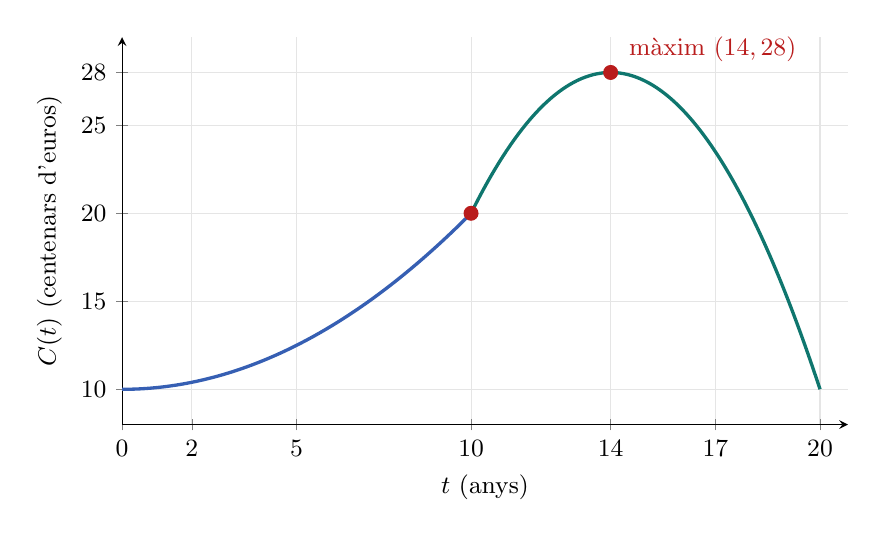
\begin{tikzpicture}
\begin{axis}[
  width=10.8cm,height=6.5cm,axis lines=left,
  xmin=0,xmax=20.8,ymin=8,ymax=30,
  xlabel={$t$ (anys)},ylabel={$C(t)$ (centenars d'euros)},
  xtick={0,2,5,10,14,17,20},ytick={10,15,20,25,28},
  grid=major,grid style={black!10},tick label style={font=\small},label style={font=\small},clip=false]
  \addplot[tramU,very thick,domain=0:10,samples=100]{x^2/10+10};
  \addplot[tramDos,very thick,domain=10:20,samples=120]{28-(x-14)^2/2};
  \addplot[only marks,mark=*,mark size=2.5pt,punt] coordinates {(10,20) (14,28)};
  \node[anchor=south west,font=\small,text=punt] at (axis cs:14.25,28.05) {màxim $(14,28)$};
\end{axis}
\end{tikzpicture}
\end{document}
